% Drawing 43/03-14 -- folder 43, batch 03, archive page 56 (PDF page 57).
% Transcription: à gauche, un segment à trois points marqués : les deux bouts et un point près du bout gauche ; la partie de droite repassée en gras.
% Kind: segment with three marked points. Method 2 (schematic redraw from the facsimile). Status: ok.
% Notes: Ink. A segment with a tick at each end and a third tick near the left end; from the third tick to the right end the stroke is heavy. Redrawn 2026-11-12 (issue 128): to check again.
% Coordinates: 1 unit = 1 mm = 1/100 of the crop width, y downwards as on the crop (bbox in page fractions: [0.21, 0.2, 0.41, 0.25]).
% Redrawn by Claude (claude-fable-5-2), issue #128, 2026-11-12; not checked by a human; not compiled (no TeX in the session).
% Rights: reproduces part of the work -- behind RENDER_TRANSCRIPTS, never published by itself.
\documentclass[tikz,border=3pt]{standalone}
\usepackage{amsmath,amssymb}
\usetikzlibrary{patterns,arrows.meta}
\tikzset{pencil/.style={black!45}, struck/.style={black!35}, mpt/.style={circle,draw,inner sep=1.3pt}, pt/.style={circle,fill,inner sep=0.9pt}, opt/.style={circle,draw,fill=white,inner sep=1.1pt}, Rd/.style={red!75!black}, Gn/.style={green!45!black}, Br/.style={brown!70!black}}
\begin{document}
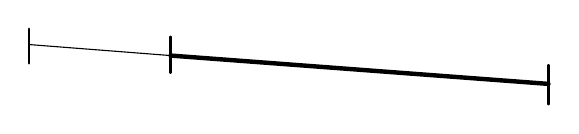
\begin{tikzpicture}[x=1mm,y=-1mm,line cap=round,line join=round,font=\small]
\coordinate (a) at (17,18);
\coordinate (b) at (35,19.4);
\coordinate (c) at (83,23);
\draw (a) -- (b);
\draw[line width=1.6pt] (b) -- (c);
\draw[thick] (17,16) -- (17,20.4);
\draw[thick] (35,17) -- (35,21.6);
\draw[thick] (83,20.6) -- (83,25.6);
\end{tikzpicture}
\end{document}
